\subsection{Mass fits}
\label{sec:dsphi:fit}
Both the \Bp and \Ds mesons have quantum numbers $J^P=0^-$, and the \phii is $1^-$ .
Therefore the decay \btodsphi is a transition of a pseudoscalar to a pseudoscalar and a vector
meson.
In order for angular momentum to be conserved, the vector particle must be produced in the $j=0$
state, where the spin is orthogonal to the particle's momentum.
Therefore, the vector \phii in the decay \btodsphi must be lonitudinally polarized in the final
state, and its daughter kaons have an angular distribution proportional to $\cos^2\thetahel$, as
shown in \Fig{fig:dsphi:hel}.
This proves to be an excellent variable for separating signal and background, because most
backgrounds are flat in $\cos\thetahel$.
It transpired that a cut of $|\cos\thetahel|>0.4$ was $93\pc$ signal efficient.

\begin{figure}
  \begin{center}
    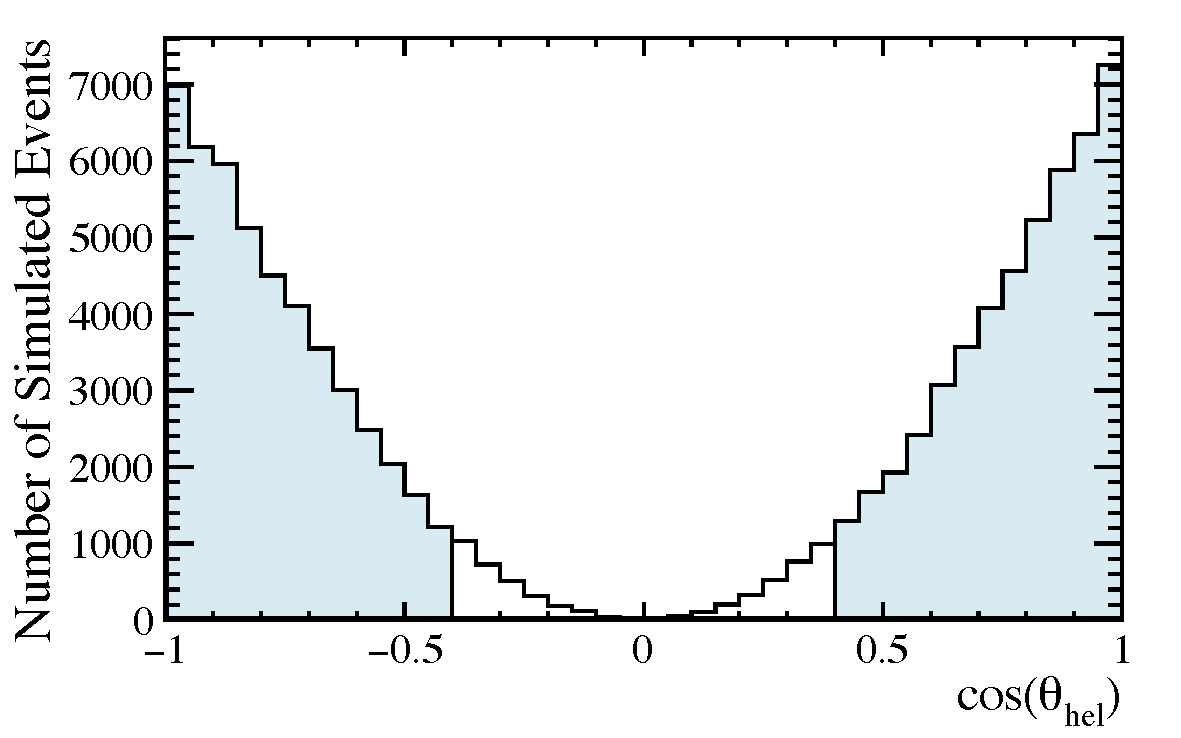
\includegraphics[width=0.48\textwidth]{thetahel}
    %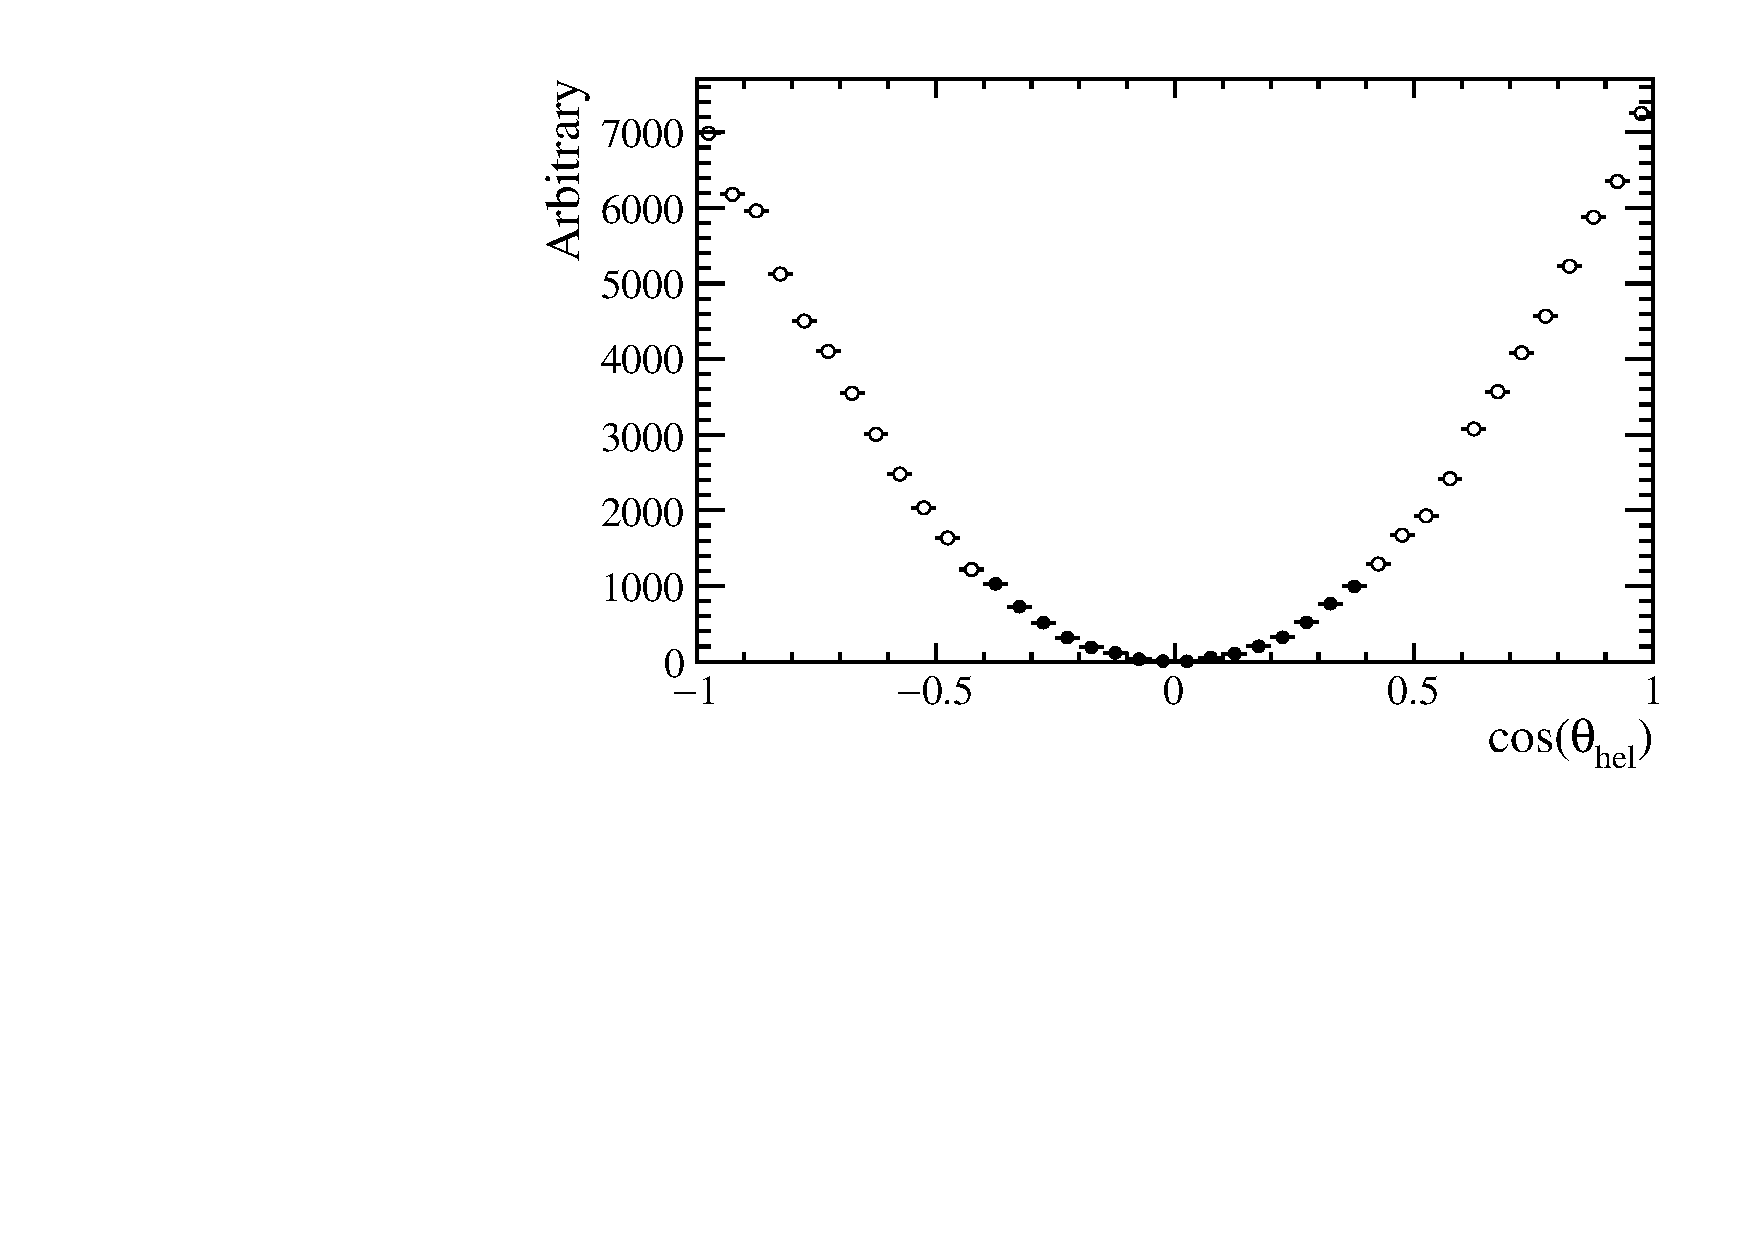
\includegraphics[width=0.48\textwidth]{thetahel2}
    \caption[Distribution of \thetahel in \btodsphi]
    {\small
      Distribution of $\cos\thetahel$, where \thetahel is the angle between the \Bp and \Kp in the
      rest frame of the \phii from simulated events.
      The shaded region indicates $|\cos\thetahel|>0.4$, which defines the signal region.
      For the decay \btodsphi, where the \Bp and \Ds mesons are both pseudoscalars, and the
      \phii is a vector, the \phii is forced into the $j=0$ state.
      Therefore, the angular distrubution of \thetahel is proportional to $\cos^2\thetahel$.
    }
    \label{fig:dsphi:hel}
  \end{center}
\end{figure}

Fit regions are further split according to the invariant mass of the \phii candidate.
A signal region is defined for \phitokk candidates with a mass within $20\mev$ of the nominal \phii
mass, and a sideband region is defined for candidates with a mass in the range
\mbox{$20<\left|m_\phi^\pdg-m_\kk\right|<40\mev$}.

The four fit regions --- defined by \thetahel and $m_{\kk}$ --- have a signal region, \rA,
containing most of the signal, and a purely background region, \rD.
Region \rB has a signal-like helicity angle, but is in the \phii sideband region, while region \rC
is the opposite.
A summary of cuts defining the four fit regions is shown in \Tab{tab:dsphi:hel}.
By simultaneously fitting \btodsphi candidates in all four regions allows regions \rB, \rC, and \rD
to help constrain the background in the signal region.
%The angle \thetahel is the helicity angle of the \phii, defined as the angle between the \Kp and
%the \Bp in the rest frame of the \phii.
%This is used to further separate the signal decay \btodsphi from other backgrounds.

\begin{table}
  \caption[Fit regions]
  {\small
    Fit regions used to search for the decay \btodsphi.
    Approximately $89\,\%$ was expected to be in region \rA.
  }
  \label{tab:dsphi:hel}
  \begin{center}
    \begin{tabular}{cccc}
      \toprule
      &&\multicolumn{2}{c}{$|m_{\kk}-m_\phi^\pdg|$ (MeV)}\\
      &&$\in[0,20]$&$\in[20,40]$ \\
      \midrule
      \multirow{2}{*}{$|\cos\thetahel|$}
      &$>0.4$ & \rA & \rB \\
      &$<0.4$ & \rC & \rD \\
      \bottomrule
    \end{tabular}
  \end{center}
\end{table}


%It transpired that a cut of $|\cos\thetahel|>0.4$ was $93\pc$ signal efficient, and combining this
%with a cut of $|\mass{\kk}-\mass{\phi}^\pdg|<20\mev$ mass defines a signal region.
%Other regions are defined with

%It is possible to remove about $93\pc$ of background by requiring that $|\cos\thetahel|>0.4$,
%this is the same cut value as used in \Ref{LHCb-PAPER-2011-008}.
%Therefore, two regions are defined in terms of $\cos\thetahel$, and both are used in a simultaneous
%fit.
%This also allows the combinatorial and peaking backgrounds to be separated from the signal because
%these do not necessarily have a longitudilnally polarized \phii.

The signal yield of the decay \btodsphi is determined with an unbinned maximum likelihood
fit performed simultaneously to the invariant mass spectrum of the candidate \Bp mesons in
the four regions defined above.
In each region of the fit, there are several components: the signal \btodsphi; combinatorial
background; and specific backgrounds that peak below the \Bp mass.
The final state particles in this analysis of the decay \btodsphi are $\kkpi\kk$, given the mass
cuts on the \Ds and \phii candidates, there are no sources of background which peak at the \Bp
mass.
However, there are backgrounds from genuine $B$-hadron decays in which a particle --- or multiple
particles --- are not reconstructed, and therefore form below the mass of the \Bp

After the selection requirements
the most significant backgrounds above $5100\mev$ of these are the decays\footnote{
  For these decays, the \Kstarz refers to the $K^*(892)^0$ meson.
}:
\begin{center}
  \begin{tabular}{llll}
    $\Bp\to$ & \Dss & \phii \\
    & \;\nlto $\Ds\gamma$ & \;\nlto $\boldsymbol{\kk}$ \\
    & \phantom{\Ds}\nlto $\boldsymbol{\kkpi}$ \\\rule{0pt}{4ex}
    $\Bsb\to$ & \Ds & \Kstarz & $\boldsymbol{\Km}$ \\
    & \;\nlto $\boldsymbol{\kkpi}$ & \;\nlto $\boldsymbol{\Kp}\pim$ \\\rule{0pt}{4ex}
    $\Bsb\to$ & \Dss & \Kstarz & $\boldsymbol{\Km}$ \\
    & \;\nlto$\Ds\gamma$ & \;\nlto$\boldsymbol{\Kp}\pim$ \\
    & \phantom{\Ds}\nlto $\boldsymbol{\kkpi}$ \\
  \end{tabular}
\end{center}
where an emboldened particle indicates a reconstructed track.
The decay \bstodskstrk has never been observed, but given that the branching fraction of the decay
$\decay{\Bd}{\Dm\Kstarzb\Kp}$ is $(8.8\pm1.9)\e{-4}$~\cite{PDG2012}, it should be in the
\btodsphi selection.
There is no contribution in the mass range of interest from the \decay{\Bd}{\Dm\Kstarzb\Kp} mode,
because of the mass difference between the \Bs and \Bd mesons.
As well as \bstodskstrk, the decay \bstodsstrkstrk was also expected to be present in the sample.
All these specific backgrounds are irreducible and must be accounted for in the fit.


\subsubsection{Contributions to the mass fit}
The signal shape of \btodsphi is described by a A Gaussian function, with a mean $\mu$ and standard
deviation $\sigma$.
Combinatorial background is modelled using a decaying exponential function.

The shape of \Bp candidates originating from the \btodsstrphi background is taken from simulated
events.
The $\phi$ from the decay \btodsstrphi does not need to be longitudinally polarized because the
\Dssp is a vector meson ($J^P=1^-$).
Therefore the background from the decay \btodsstrphi contributes in all fit regions.
Since the shapes of these reconstructed candidates are non-trivial, a kernel density estimation
technique~\cite{Cranmer:2000du} is used to describe the shape.
Figure~\ref{fig:dsphi:sigshape} shows the kernelized distribution for the whole set of simulated
events, as well as each individual helicity region.
It was assumed that \Dssp was unpolarized, as observed in many other cases where a
$B$ decays into a vector-vector final state.
Despite this, different \phii polarizations caused the shape of the distribution to differ
between the two helicity regions.

\begin{figure}
  \begin{center}
    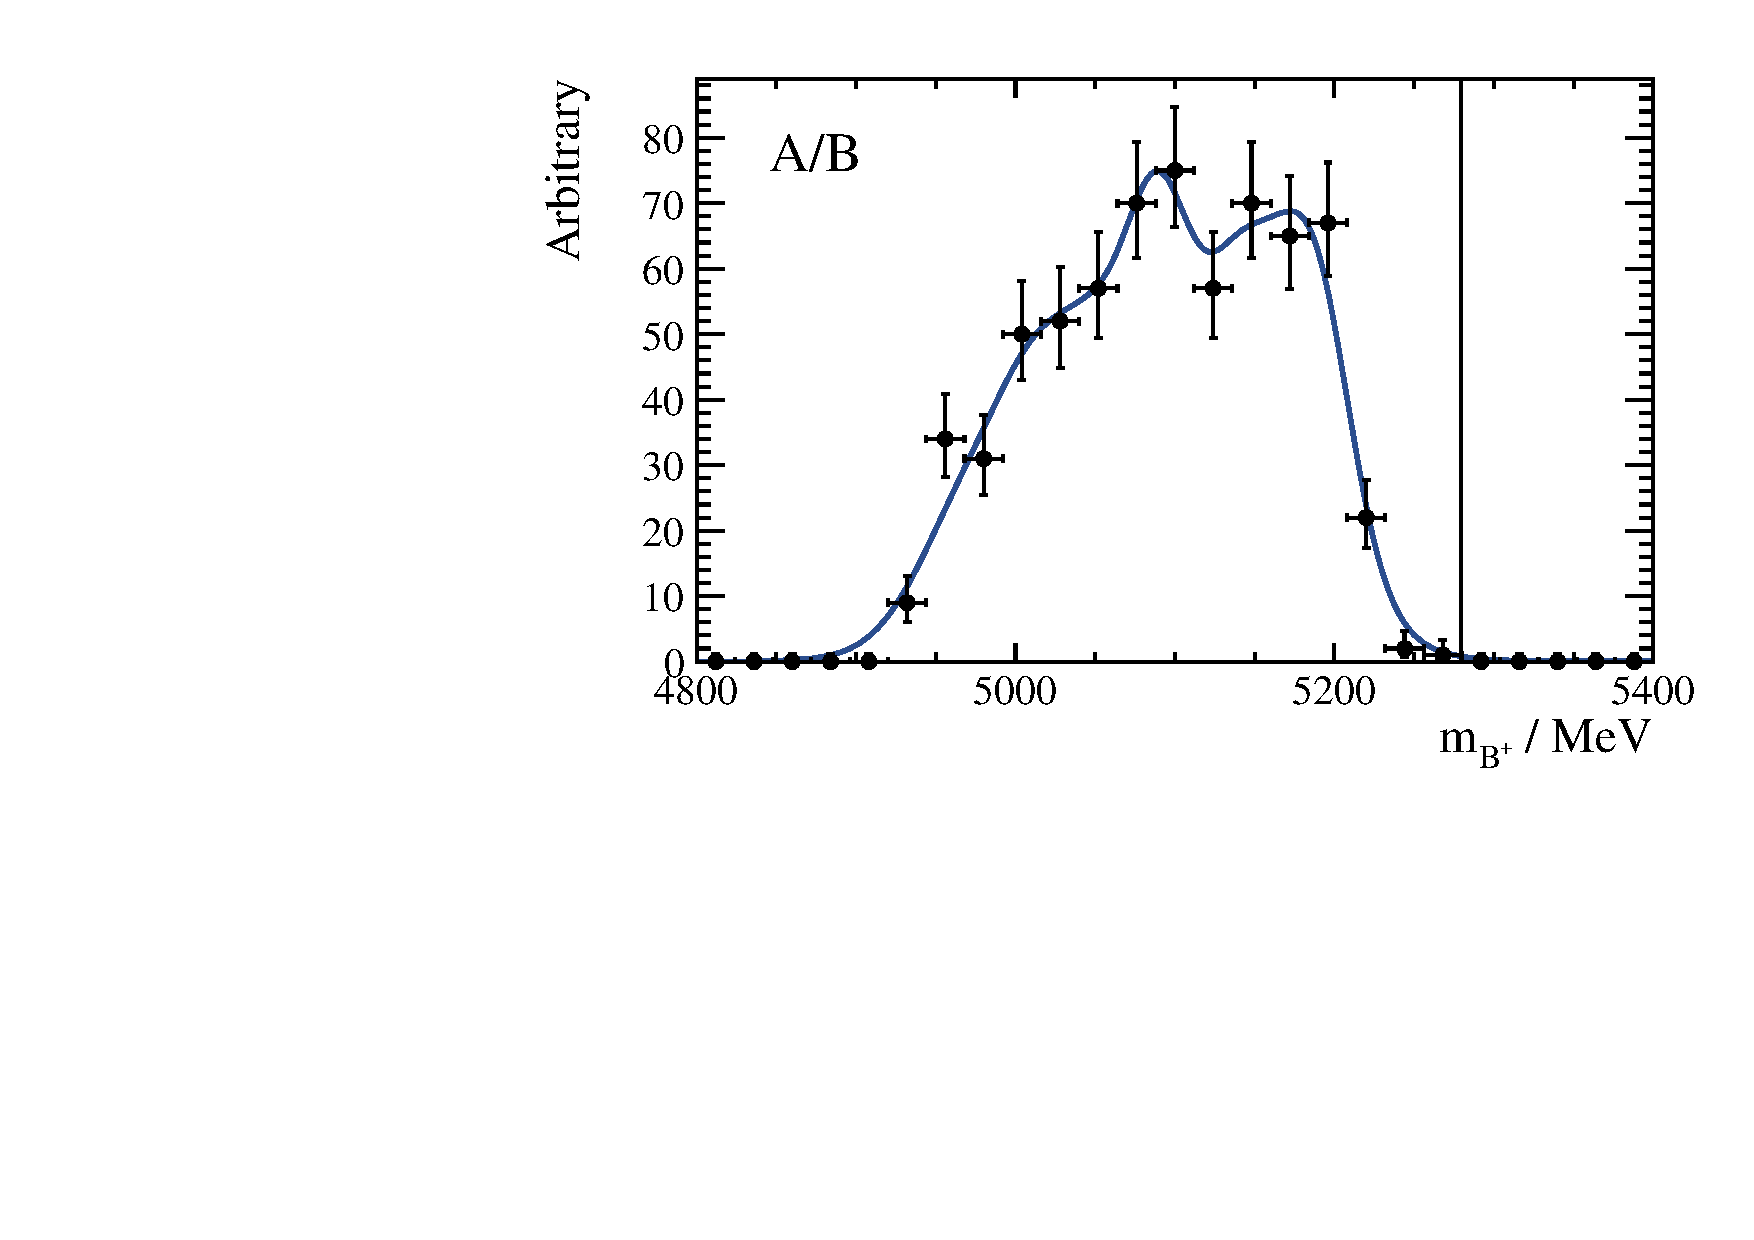
\includegraphics[width=0.48\textwidth]{b2dsstrphi_sig}
    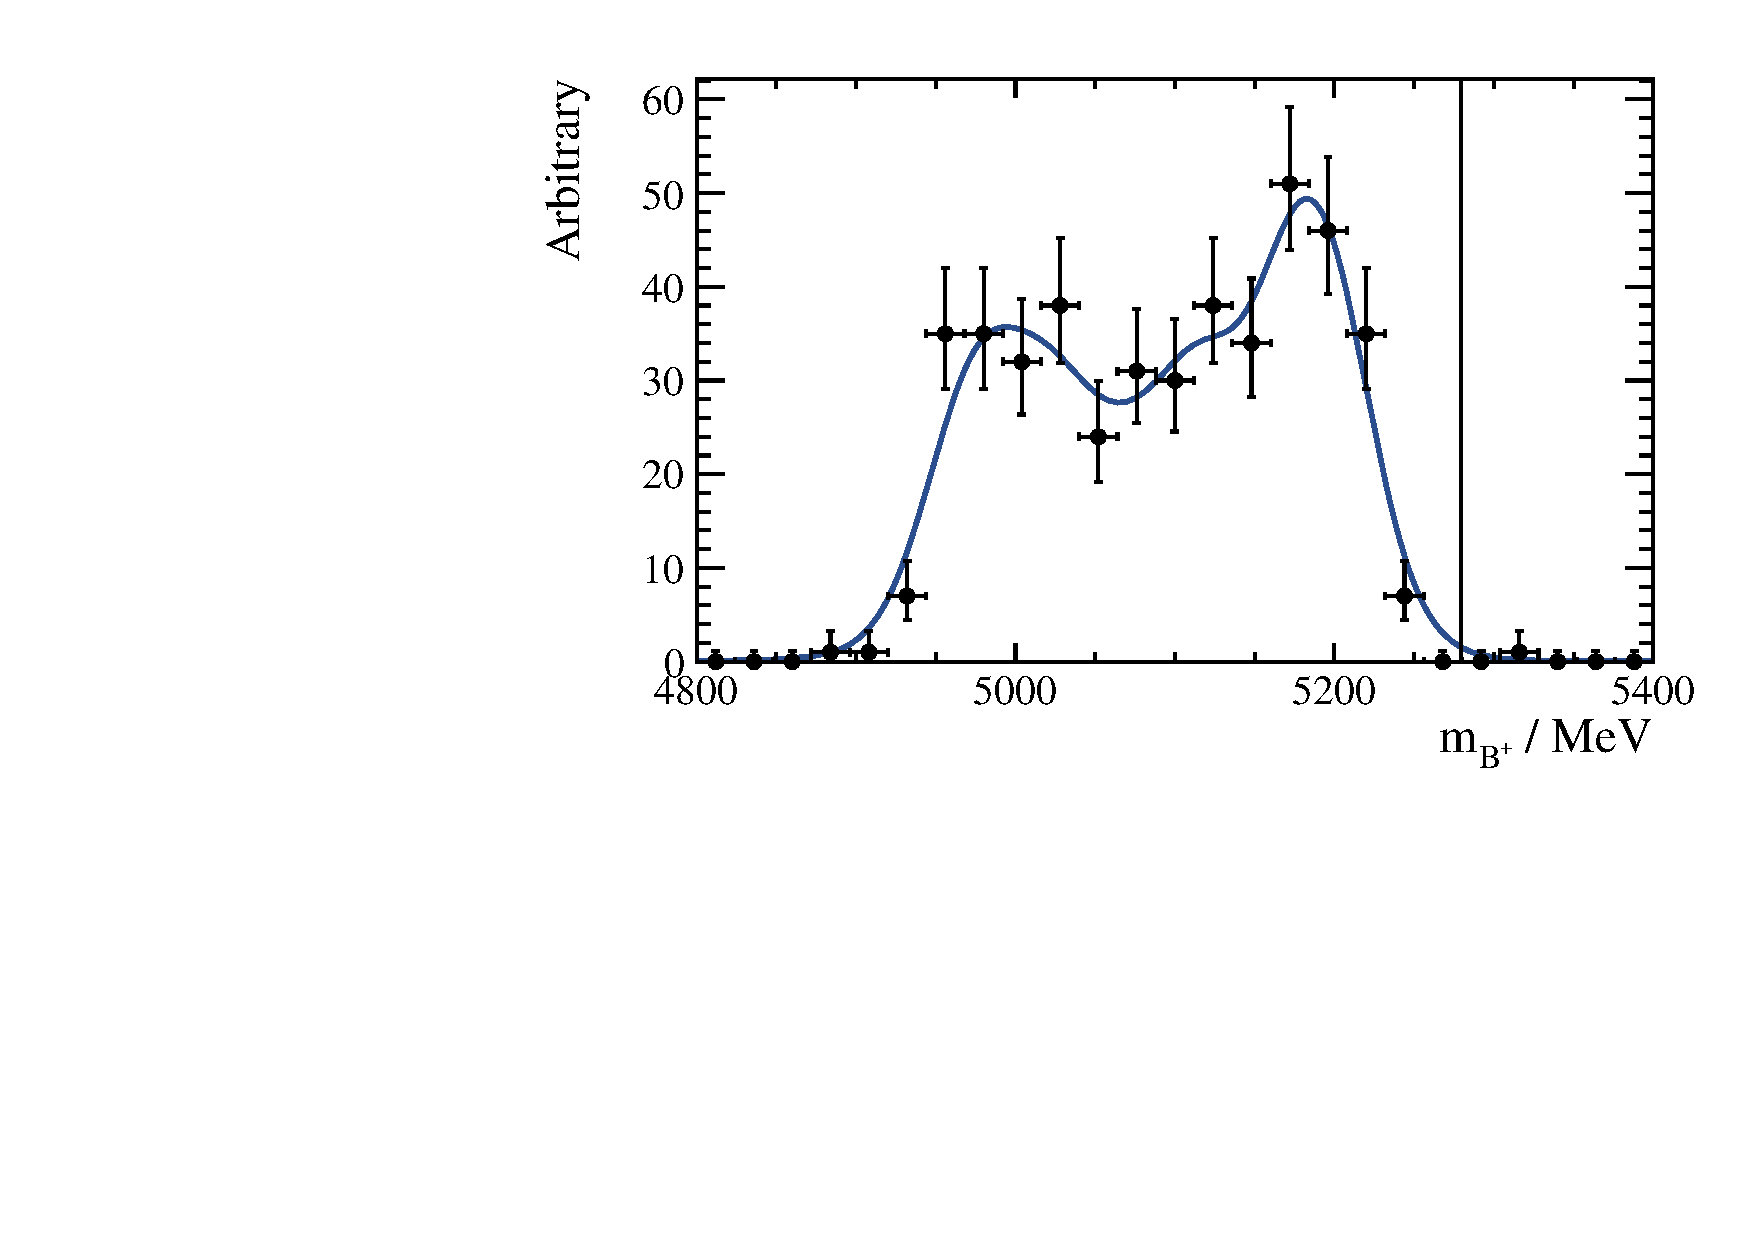
\includegraphics[width=0.48\textwidth]{b2dsstrphi_hel}\\
    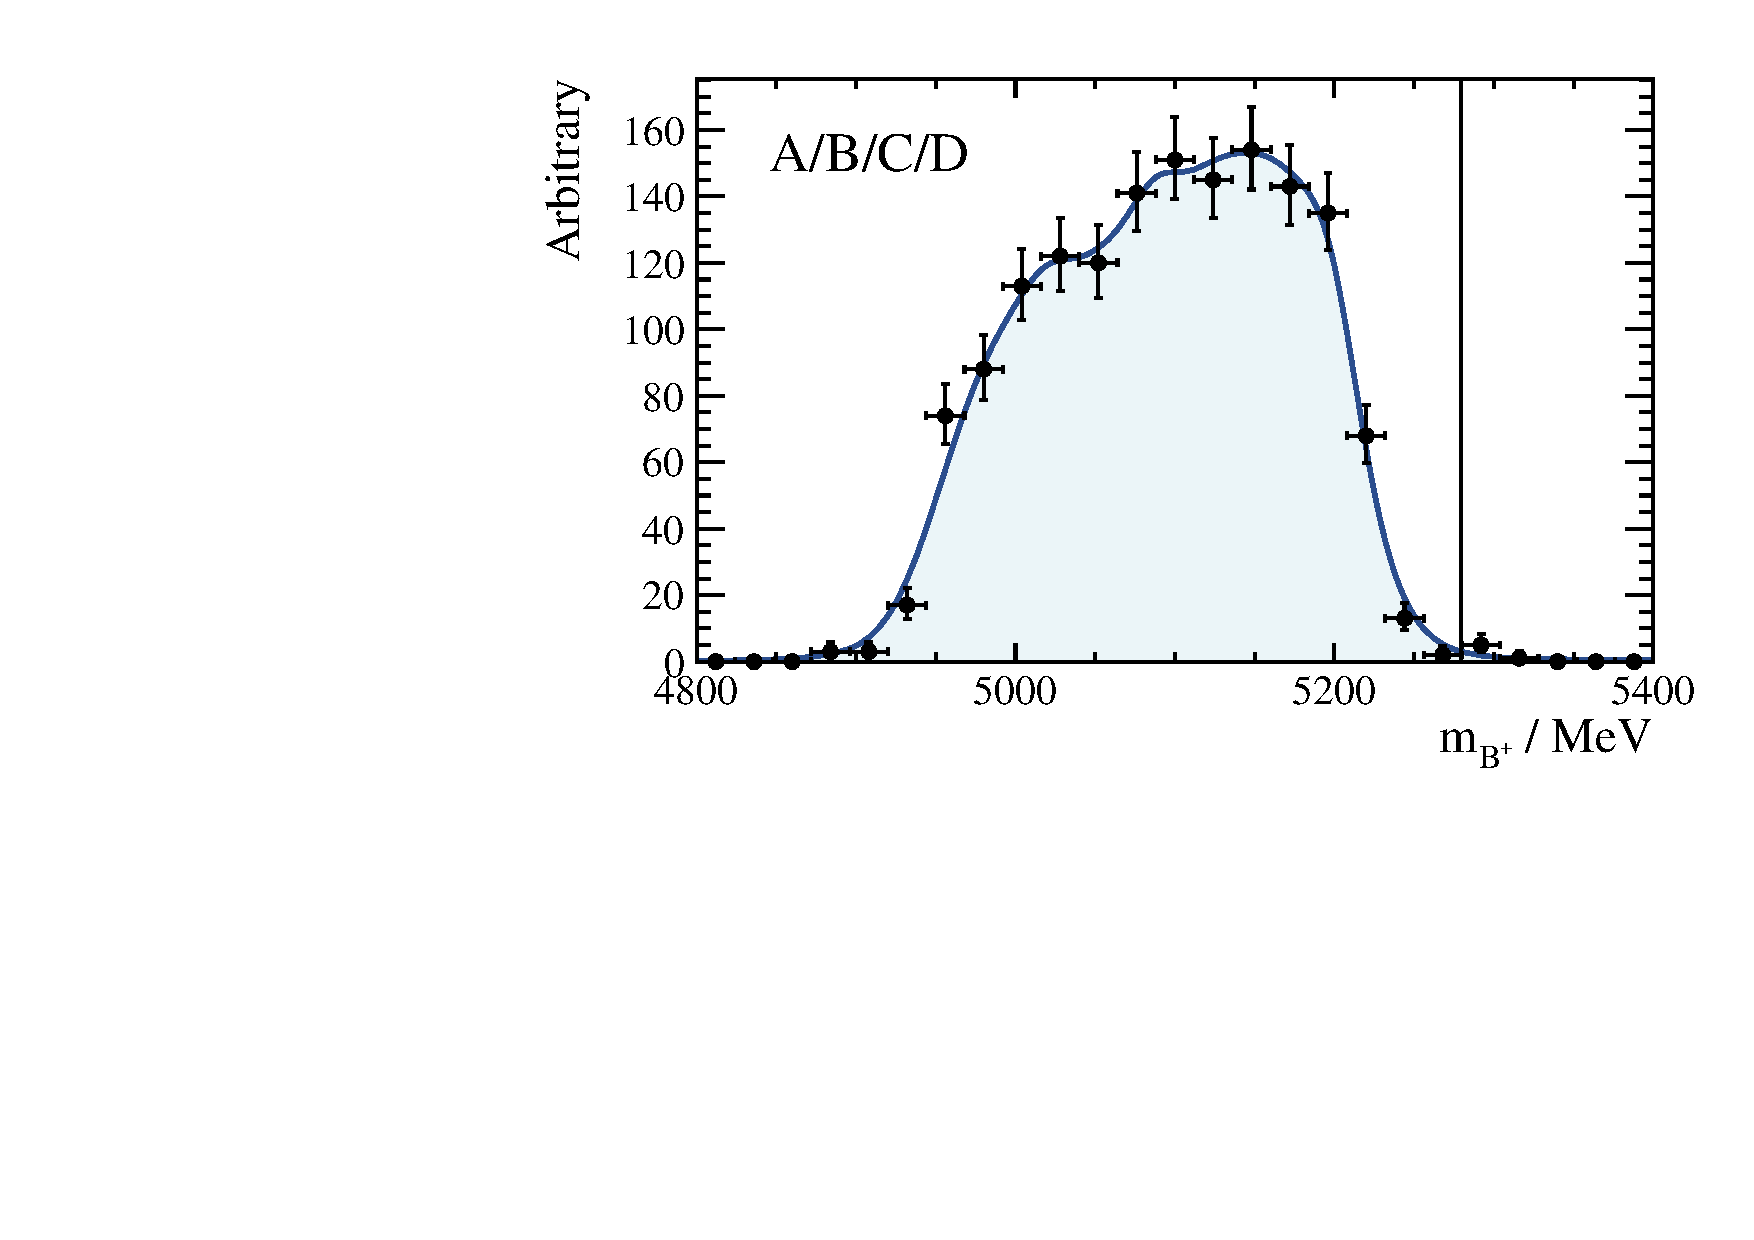
\includegraphics[width=0.48\textwidth]{b2dsstrphi_both}
    \caption[Contribution to the \btodsphi fit from the \btodsstrphi background]
    {
      Distributions of the invariant mass distribution of simulated events of \btodsstrphi
      in the indicated fit regions and the resulting kernelized function.
      The shape of these background distributions varies depending on the helicity cut, but the
      rising edge on the right hand side is the same in each case.
      In the fit to the data, the distribution made from all events.
      The vertical line indicates the \Bp mass.
    }
    \label{fig:dsphi:dsstrphi}
  \end{center}
\end{figure}



%Therefore the value of $\cos\thetahel$ is uniformly
%distributed between zero and one.
%The photon from the decaying \Dssp is not reconstructed, and therefore the background from the
%decay \btodsstrphi peaks below the nominal \Bp mass.
%The decay \btodsstrkstrk has never been observed


%Other sources of background that peak below the mass of the \Bp meson are from the decay modes
%$\decay{\Bsb}{D_s^{(*)+}\Kstarz\Km}$.
%These arise when the pion from the \decay{\Kstarz}{\Kp\pim} is not reconstructed.
%Since there is missing energy from the pion (and photon in the case of the \Dssp decay), these peak
%significantly below the \Bp mass.

Backgrounds from the decay \bstodskstrk result in highly non-trivial invariant mass shapes when the
\pip from the \Kstarz decay is missed.
Once again, kernel density estimation techniques~\cite{Cranmer:2000du} were used to get an
understanding of the background shape.
Due to the low statistics, simulated \bstodskstrk events falling in regions \rA and \rB are used to
make the background distributions, and then shifted up by $35\mev$ for regions \rC and \rD.
The value of $35\mev$ is an amount that was observed from data, and due to the shape of the \kk
S-wave under the \phii mass peak.
These shapes are shown in \Fig{fig:dsphi:bstodskstrk}.

\begin{figure}
  \begin{center}
    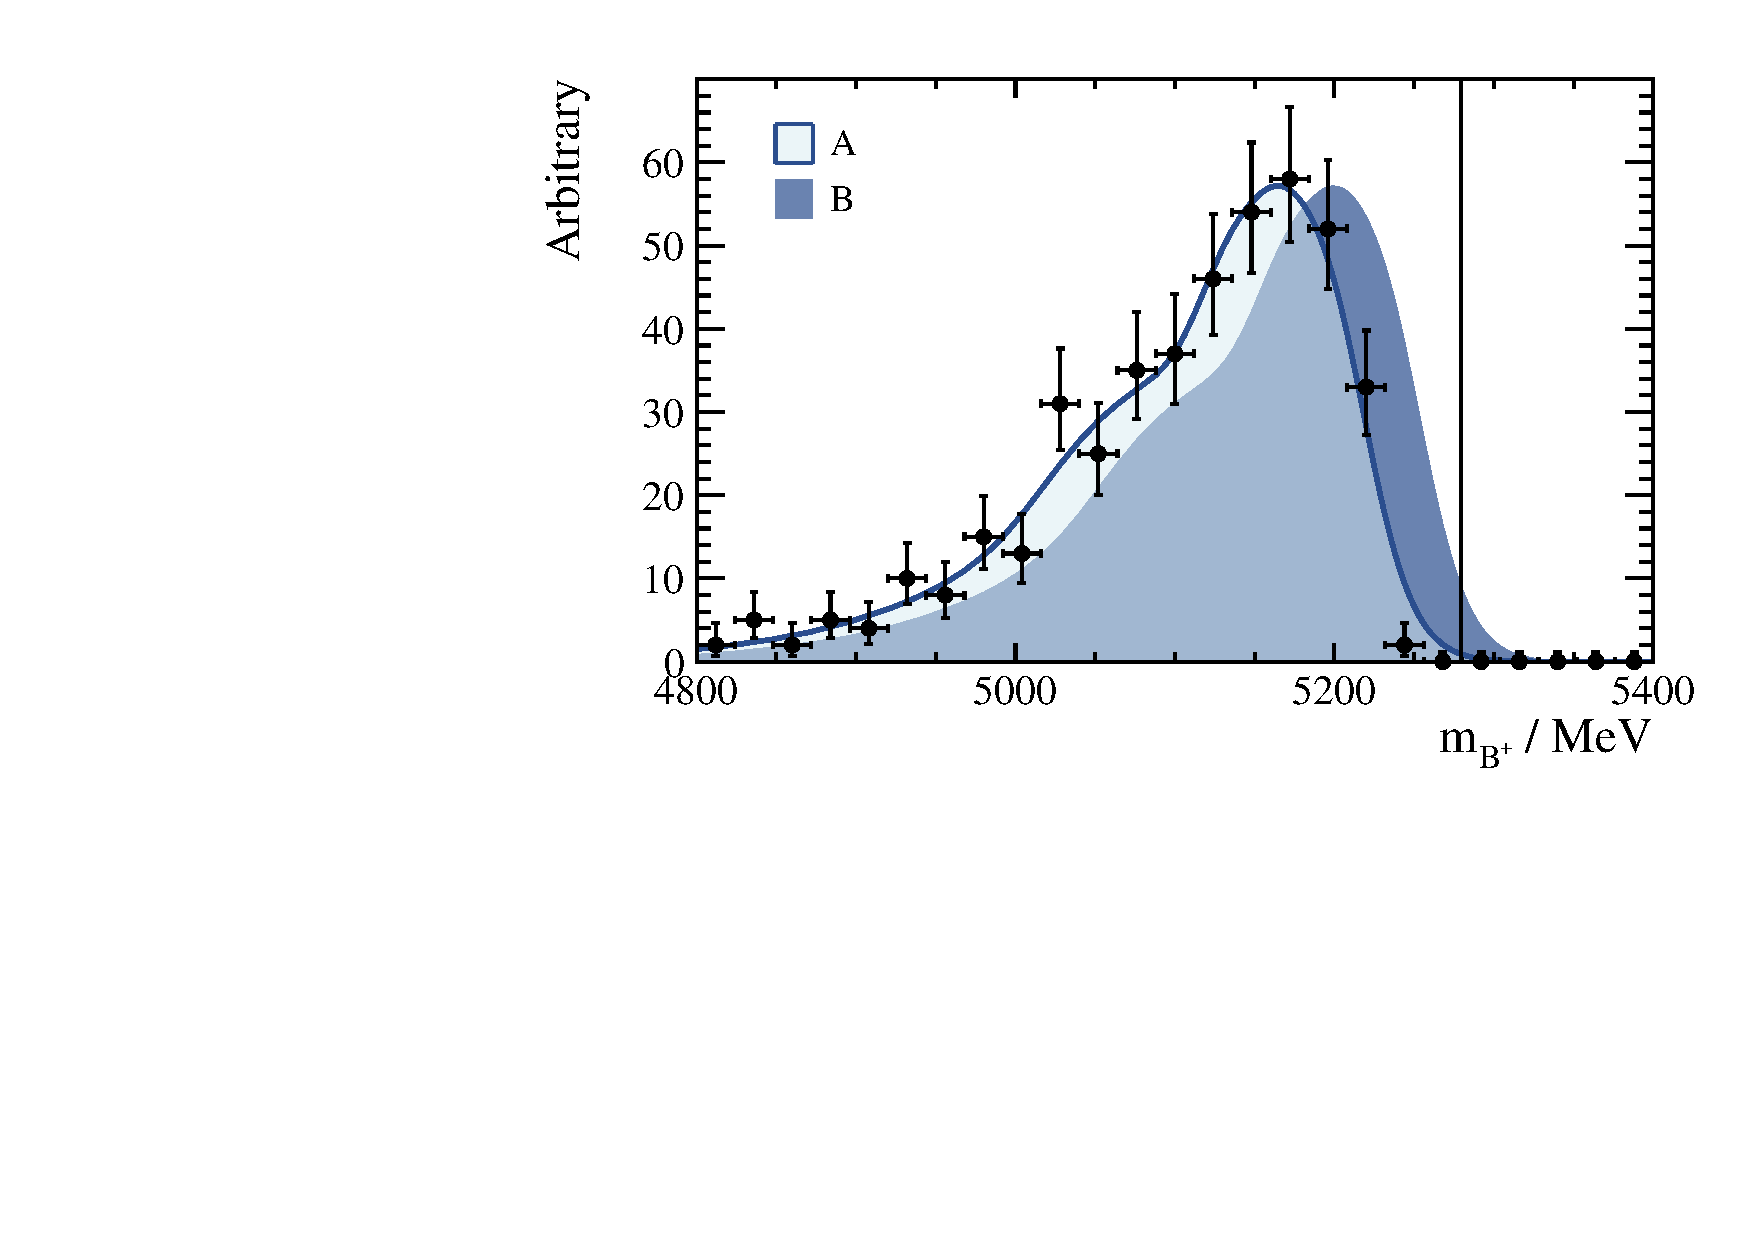
\includegraphics[width=0.48\textwidth]{bs2dskkstr_sig}
    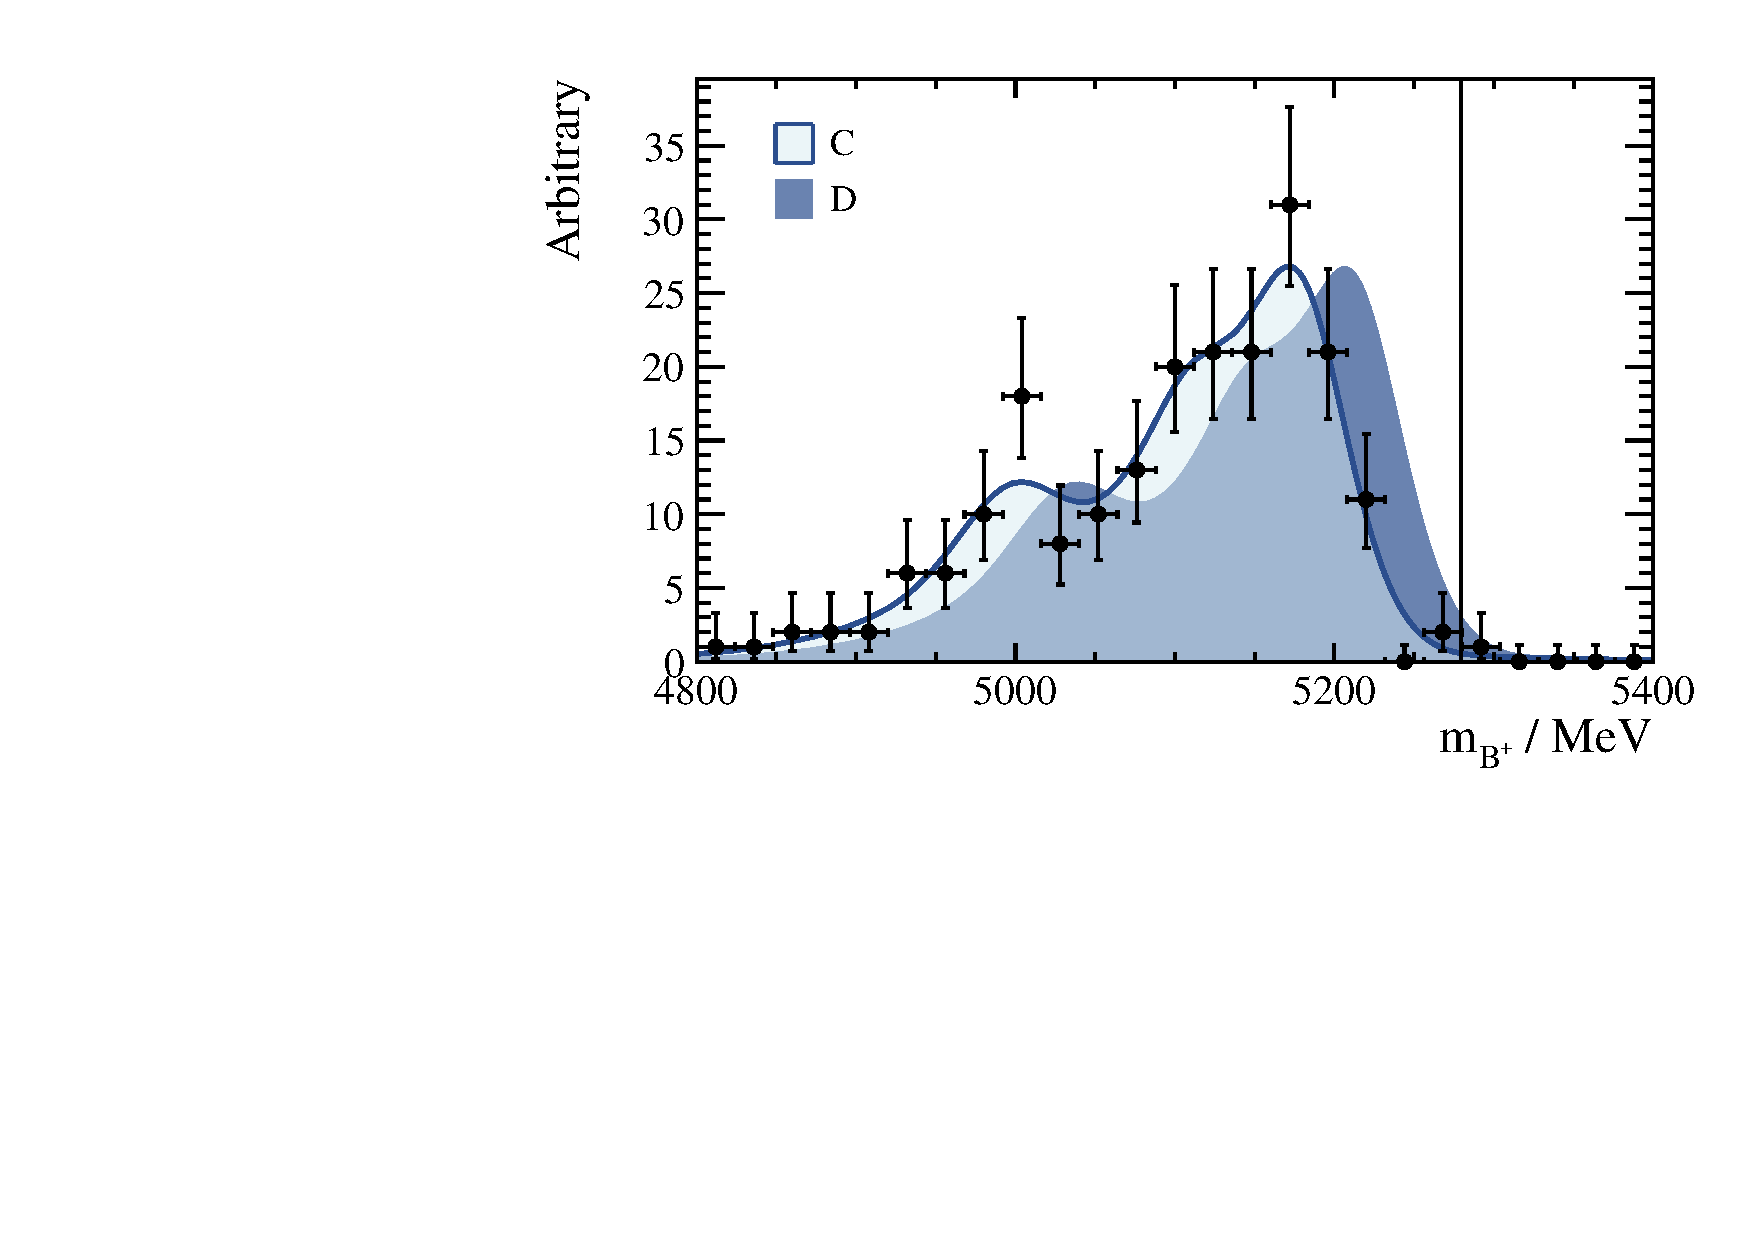
\includegraphics[width=0.48\textwidth]{bs2dskkstr_hel}
    \caption[Shapes of background contributions of \bstodskstrk]
    {\small
      Distributions of the invariant mass distribution of simulated events of \bstodskstrk in the
      (left) signal helicity regions \rA and \rB, and
      (right) background helicity regions \rC and \rD.
      The pale blue shapes at lower mass are from the the signal region in $m_\kk$, and the dark
      shapes are shifted up in mass by $35\mev$ to model the \phii mass sidebands.
    }
    \label{fig:dsphi:bstodskstrk}
  \end{center}
\end{figure}

An estimate of the shape of the background distribution of \bstodsstrkstrk is estimated by taking
the simulated \bstodskstrk events, shifting them down in mass and smearing to account for the
additional missing \photon from the \Dss decay.
There is $5\mev$ increase in the mean of the background in the \phii sideband regions.
This shape is shown in \Fig{fig:dsphi:bstodsstrkstrk}.

\begin{figure}
  \begin{center}
    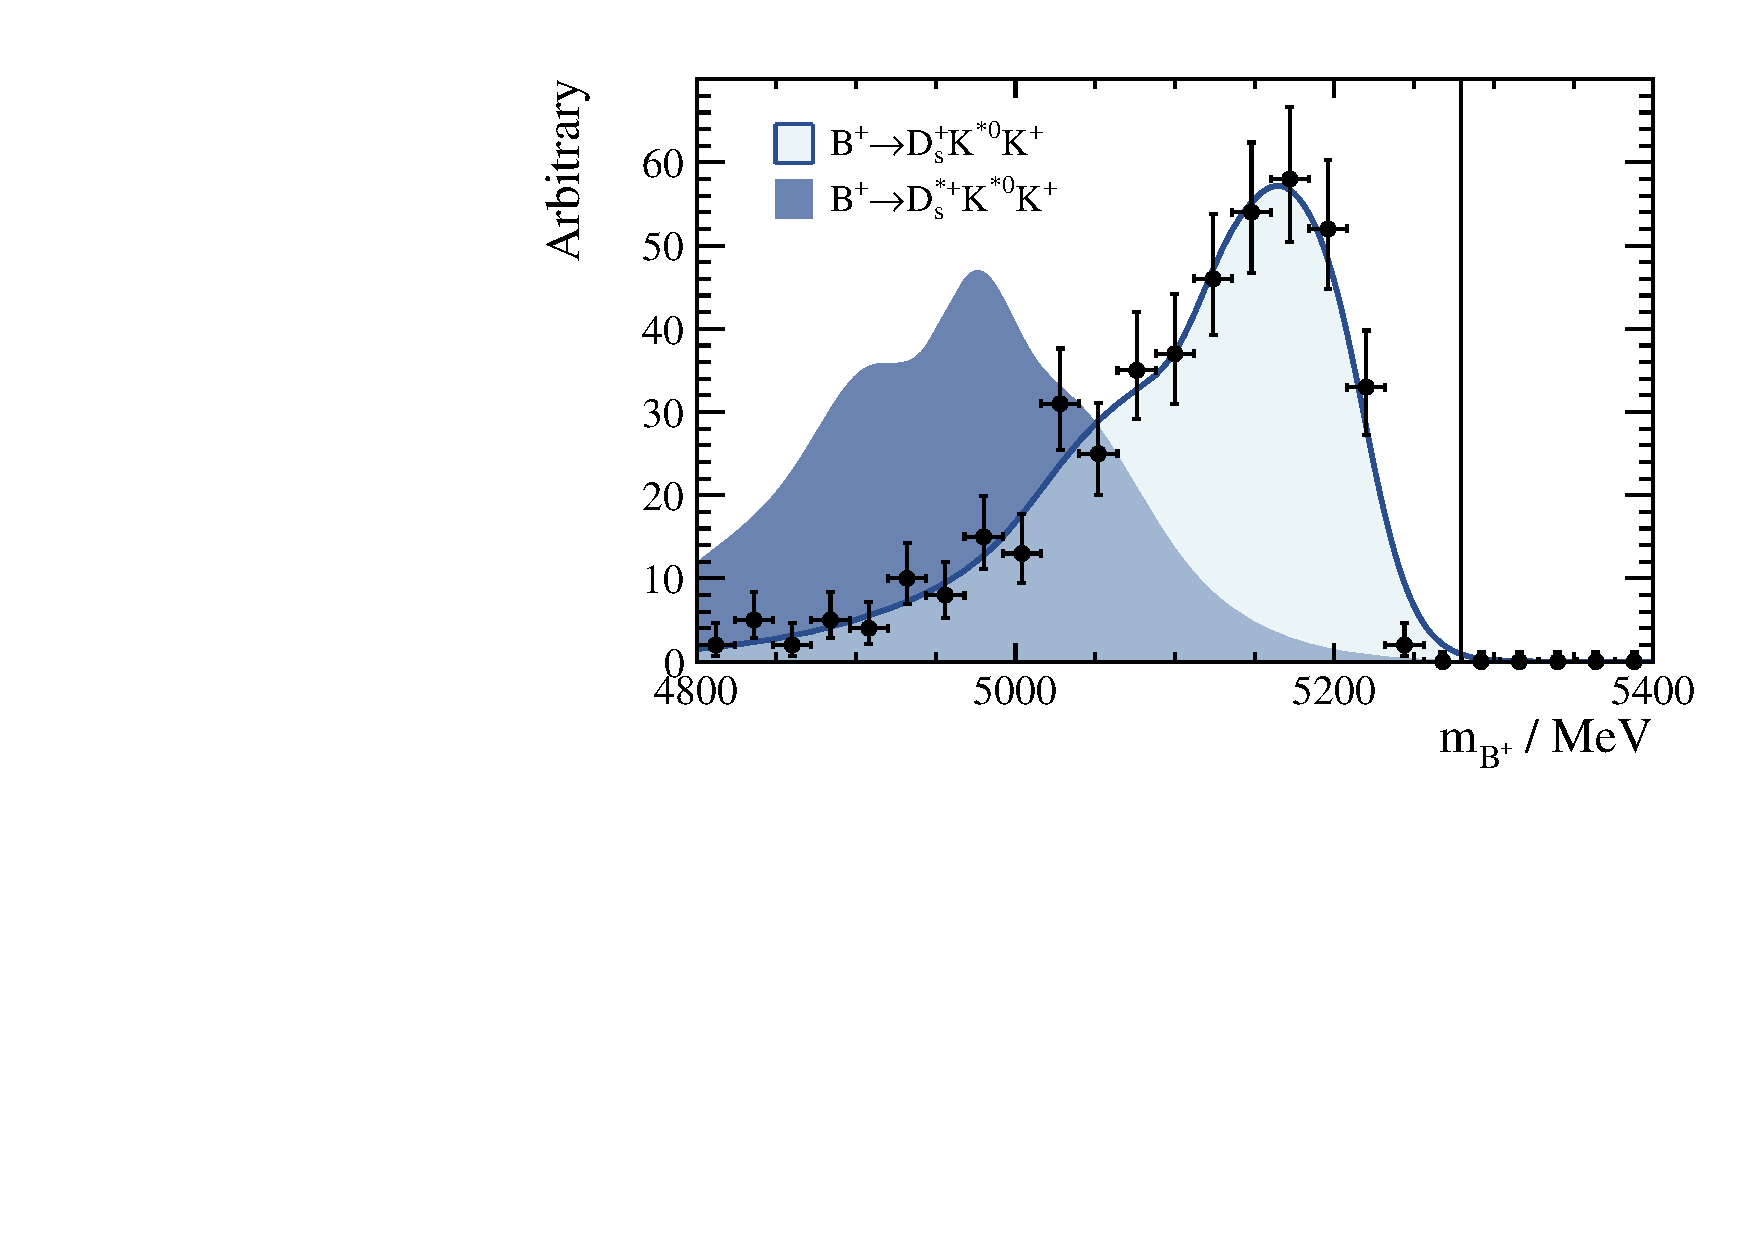
\includegraphics[width=0.48\textwidth]{bs2dsstrkstrk}
    \caption[Shapes of background contributions of \bstodsstrkstrk]
    {\small
      Distribution of the \bstodsstrkstrk background shape, in regions \rA and \rB, relative to
      that of the \bstodskstrk from region \rA.
      The \bstodsstrkstrk background in \rC and \rD are the same as those shown, but shifted up in
      mass by $5\mev$.
      The shape of the \bstodsstrkstrk background is made by shifting the displayed data down in
      mass and smearing to account for the additional lost photon from the \Dss.
      This resulting shape is then kernelized.
      The vertical line indicates the \Bp mass.
    }
    \label{fig:dsphi:bstodsstrkstrk}
  \end{center}
\end{figure}

As mentioned previously, the decays \bstodskstrk and \bstodsstrkstrk have never been observed, but
are expected to contribute.
The shape for \bstodskstrk is taken directly from kernelized simulated events.
There were no simulated events available with which to understand the shape of the \bstodsstrkstrk
background.
Instead the shape taken from the \bstodskstrk background is convolved with a distribution
parameterizing the loss of a photon (or pion) as seen between the decays \btodsstrphi and
\bstodskstrk.




\subsubsection{Constraints on the fit}
The mass fit constitutes a simultaneous fit to four regions, in each of which there are four
background distributions as well as a signal component (a total of at least 32 free parameters).
Clearly this is very challenging, especially considering that there are low statistics and complex
background models.
It is therefore necessary to use relationships --- derived from simulation or data --- to fix as
many parameters as possible.
The following section will outline how the shape of each distribution is derived and how different
parameter are constrained.

The signal Gaussian function,
has a value of $\sigma$ is determined to be $11\mev$ from simulation, which is then scaled up by
$20\pc$ to account for differences in resolution between simulation and data.
The mean, $\mu$, is fixed to be $5283\mev$, which is the mean mass observed in
\decay{\Bp}{\Dz\pip} (and also observed in the \Bs mode).
It is also determined from simulation that the total signal is distributed between the regions:
\rA 89\pc, \rB 4\pc, \rC 7\pc, and in \rD there is negligible expected signal contribution.
Therefore, in the following, \rA and \rD may be referred to as the signal and background regions,
respectively.

It was expected from simulation that $\sim7$ events from the decay \btodsstrphi contribute to the
background of the four fit regions, spread over $\sim300\mev$.
At this level, the difference in the true distributions and those shown in \Fig{fig:dsphi:dsstrphi}
--- especially considering rising shape is the same for all polarizations of the \phii ---
leads to a negligible difference in yield.
For this reason, the longitudinally polarized \btodsstrphi component was used in all regions of the
fit.
Just as was done with the signal component, the ratios between yields of each fit region was fixed
using simulation.
Approximately $95\pc$ of the contribution from the decay \btodsstrphi is expected to be in the
signal region.

Yields from the decays \bstodskstrk and \bstodsstrkstrk can, clearly, not be estimated.
Especially since the yield from the decay \bstodskstrk is highly sensitive to the width of the
$a_1(1260)$ --- because it decays via $a_1(1260)^+\Kstarz\Kp$ --- which is poorly
known~\cite{PDG2012}.
However, the ratios of yields in each fit regions for the decay \bstodskstrk can be determined
using simulated events.
The ratios between the yields from regions \rA/\rB and \rC/\rD was found to be $0.5\pm0.24$, and
between the regions \rA/\rC and \rB/\rD was determined to be $1.50\pm.034$.
These values are used as Gaussian constraints in the fit.

The ratio of branching fractions
\begin{equation}
  \frac{\BF\big(\decay{\Bdb}{\Dp\Kstarz\Km}\big)}
  {\BF\big(\decay{\Bdb}{\Dstarp\Kstarz\Km}\big)}
  \sim 1.5,
\end{equation}
and it is reasonable to expect the same to be true for the branching fraction ratio for the
\bstodskstrk and \bstodsstrkstrk modes.
Therefore, the ratio of yields for each region is fixed to $1.5$.

%The background shapes for \btodsstrphi and \bstodskstrk are taken from simulated events,
%reconstructed as \btodsphi candidates.
%Since the shapes of these reconstructed candidates are non-trivial, a

%The shapes of peaking background contributions are taken from kernel density
%estimates of simulated events, as described.
%Yields of background components are also fixed from...
%Therefore, the only floating parameters in the simultaneous fit is the total signal yield and the
%combinatorial background yields and shape.
%However the combinatorial background between regions is fixed.

The last remaining background component to be constrained is that of the combinatorial background,
which is modelled with a decaying exponential function.
Since the distribution of $\cos\thetahel$ is flat for combinations of random tracks, the yields
between the regions \rA/\rC and \rB/\rD  are fixed to $1.5$,
The value of the slope is Gaussian constrained to a fit across a wider range of mass in data.

A summary of all constraints in the fit model, and fit yields, are given in
\Table{fig:tab:constraints}.

\begin{table}
  \caption[Constraints applied to the fit to \btodsphi data]
  {\small
    Fit parameters used in in the fit to determine the yield of the decay \btodsphi.
    A label of $f$, means that the value is fixed in the fit; and labels of $s$ and $d$ mean
    constrained using simulated events and data over a wider mass range, respectively.
    %The yield of the background from \bstodsstrkstrk is also fixed to be $67\pc$ of
    %$N\big(\bstodskstrk\big)$
    The use of {\bf R} for the constraints of \bstodsstrkstrk indicate that it applies in each
    fit region separately.
  }
  \label{fig:tab:constraints}
  \begin{center}
    \begin{tabular}{cccc}
      \toprule
      Fit component & Parameter & Value & \\
      \midrule
      \btodsphi
      & yield \rA & $6.00\pm2.70$\\
      & \rB/\rA   & $0.044$ & $f$ \\
      & \rC/\rA   & $0.075$ & $f$ \\
      & \rD/\rA   & $0.003\pc$ & $f$ \\
      & $\mu$     & $5283\mev$ & $f$\\
      & $\sigma$     & $13.2\mev$ & $f$\\
      \littlerule
      \btodsstrphi
      & yield \rA & $8.67\pm7.36$\\
      & \rB/\rA   & $0.044$ & $f$ \\
      & \rC/\rA   & $0.00\pm0.12$\\
      & \rD/\rC   & $0.044$ & $f$ \\
      \littlerule
      \bstodskstrk
      & yield \rA & $4.94\pm1.29$\\
      & \rA/\rB, \rC/\rD & $0.50\pm0.24$ & $s$ \\
      & \rA/\rC, \rB/\rD & $1.50\pm0.34$ & $s$ \\
      \littlerule
      \bstodsstrkstrk
      & $\displaystyle{\frac{\mathrm{yield}\;{\bf R}}{\mathrm{yield}(\bstodskstrk)\;{\bf R}}}$
      & 1.5& $f$ \\
      \littlerule
      Combinatorial
      & yield \rA & $24.0\pm6.7$\\
      & yield \rB & $16.5\pm6.0$ \\
      & \rA/\rC & 1.5 & $f$\\
      & \rB/\rD & 1.5 & $f$ \\
      & exponent & $-(1.8\pm0.2)\e{-3}$ & $d$ \\
      \bottomrule
    \end{tabular}
  \end{center}
\end{table}

